\chapter{Introduction}
\chapterquote{GROMACS reminds you: “On average, it takes twenty years for the world's largest super computer to shrink down to the size of your laptop.” (Pete Beckman)}

\newpage
\section{Background: Membrane targeting to fight AMR.}
As scientists, we are always striving to make a meaningful impact on society through our work. Still, it is not always possible to find a definitive solution to the problem at hand. Despite that, every effort in building new knowledge plays a role in moving toward the final goal. This project was envisioned with this idea in mind, aiming to provide the scientific community with new tools to deepen our understanding of cyclic peptides (CPs) in order to combat one of humanity's greatest threats in the years to come: antimicrobial resistance (AMR).

The World Health Organization (WHO) has declared AMR as one of the top global public health concerns of the 21st century, linking it to an estimated 1.27 million deaths in 2019 and projecting up to 10 million deaths per year by 2050 if adequate action is not taken \cita{Murray2022}\textsuperscript{,}\cita{Tang2023}. AMR is a natural process driven by genetic changes, which lead to microorganisms no longer responding to antimicrobial medicines. Consequently, antibiotics lose their effectiveness, and infections become difficult or impossible to treat \cita{WHO}.

Conventional antibiotics, in general, exert their activity by binding to specific receptors, inhibiting the proliferation of microorganisms \cita{Lohner2009}. Because these targets can often evade antibiotic action through mutational or adaptive mechanisms, resistance readily emerges. Therefore, the development of new antimicrobial agents and therapies that aim at novel molecular candidates is a crucial aspect of this field \cita{Ahmed2024}. In this context, advances in lipidomics have revealed the bacterial membrane as a complex and tightly regulated system. Although bacterial membranes differ from eukaryotic ones at multiple levels, including overall organization and morphology, differences in lipid composition provide a particularly tractable basis for selective antimicrobial strategies. The differences in lipidic composition between eukaryotic and bacterial membranes open the possibility of exploiting the lipidic composition as a molecular target \cita{Sani2015}. While eukaryotic cell membranes are mainly formed by phosphatidylcholine (PC), representing 50\% of the lipids, and phosphatidylserine (PS), particularly abundant in the inner leaflet, the most abundant lipids in bacteria are phosphatidylglycerol (PG) and phosphatidylethanolamine (PE) \cita{Geiger2013}\textsuperscript{,}\cita{Vance2015}. As can be seen in Figure \ref{fig:Lipids}, PG and PS are anionic polar heads, whereas PC and PE carry zero net charge. The asymmetric lipid distribution in eukaryotic membranes results in a neutral surface charge \cita{Ikeda2006}, whereas bacterial membranes are generally negatively charged due to the presence of PG. Therefore, molecules that can be attracted by this negative charge can be good candidates to use bacteria lipid composition as molecular target.
\FloatBarrier
\begin{figure}[h]
    \centering
    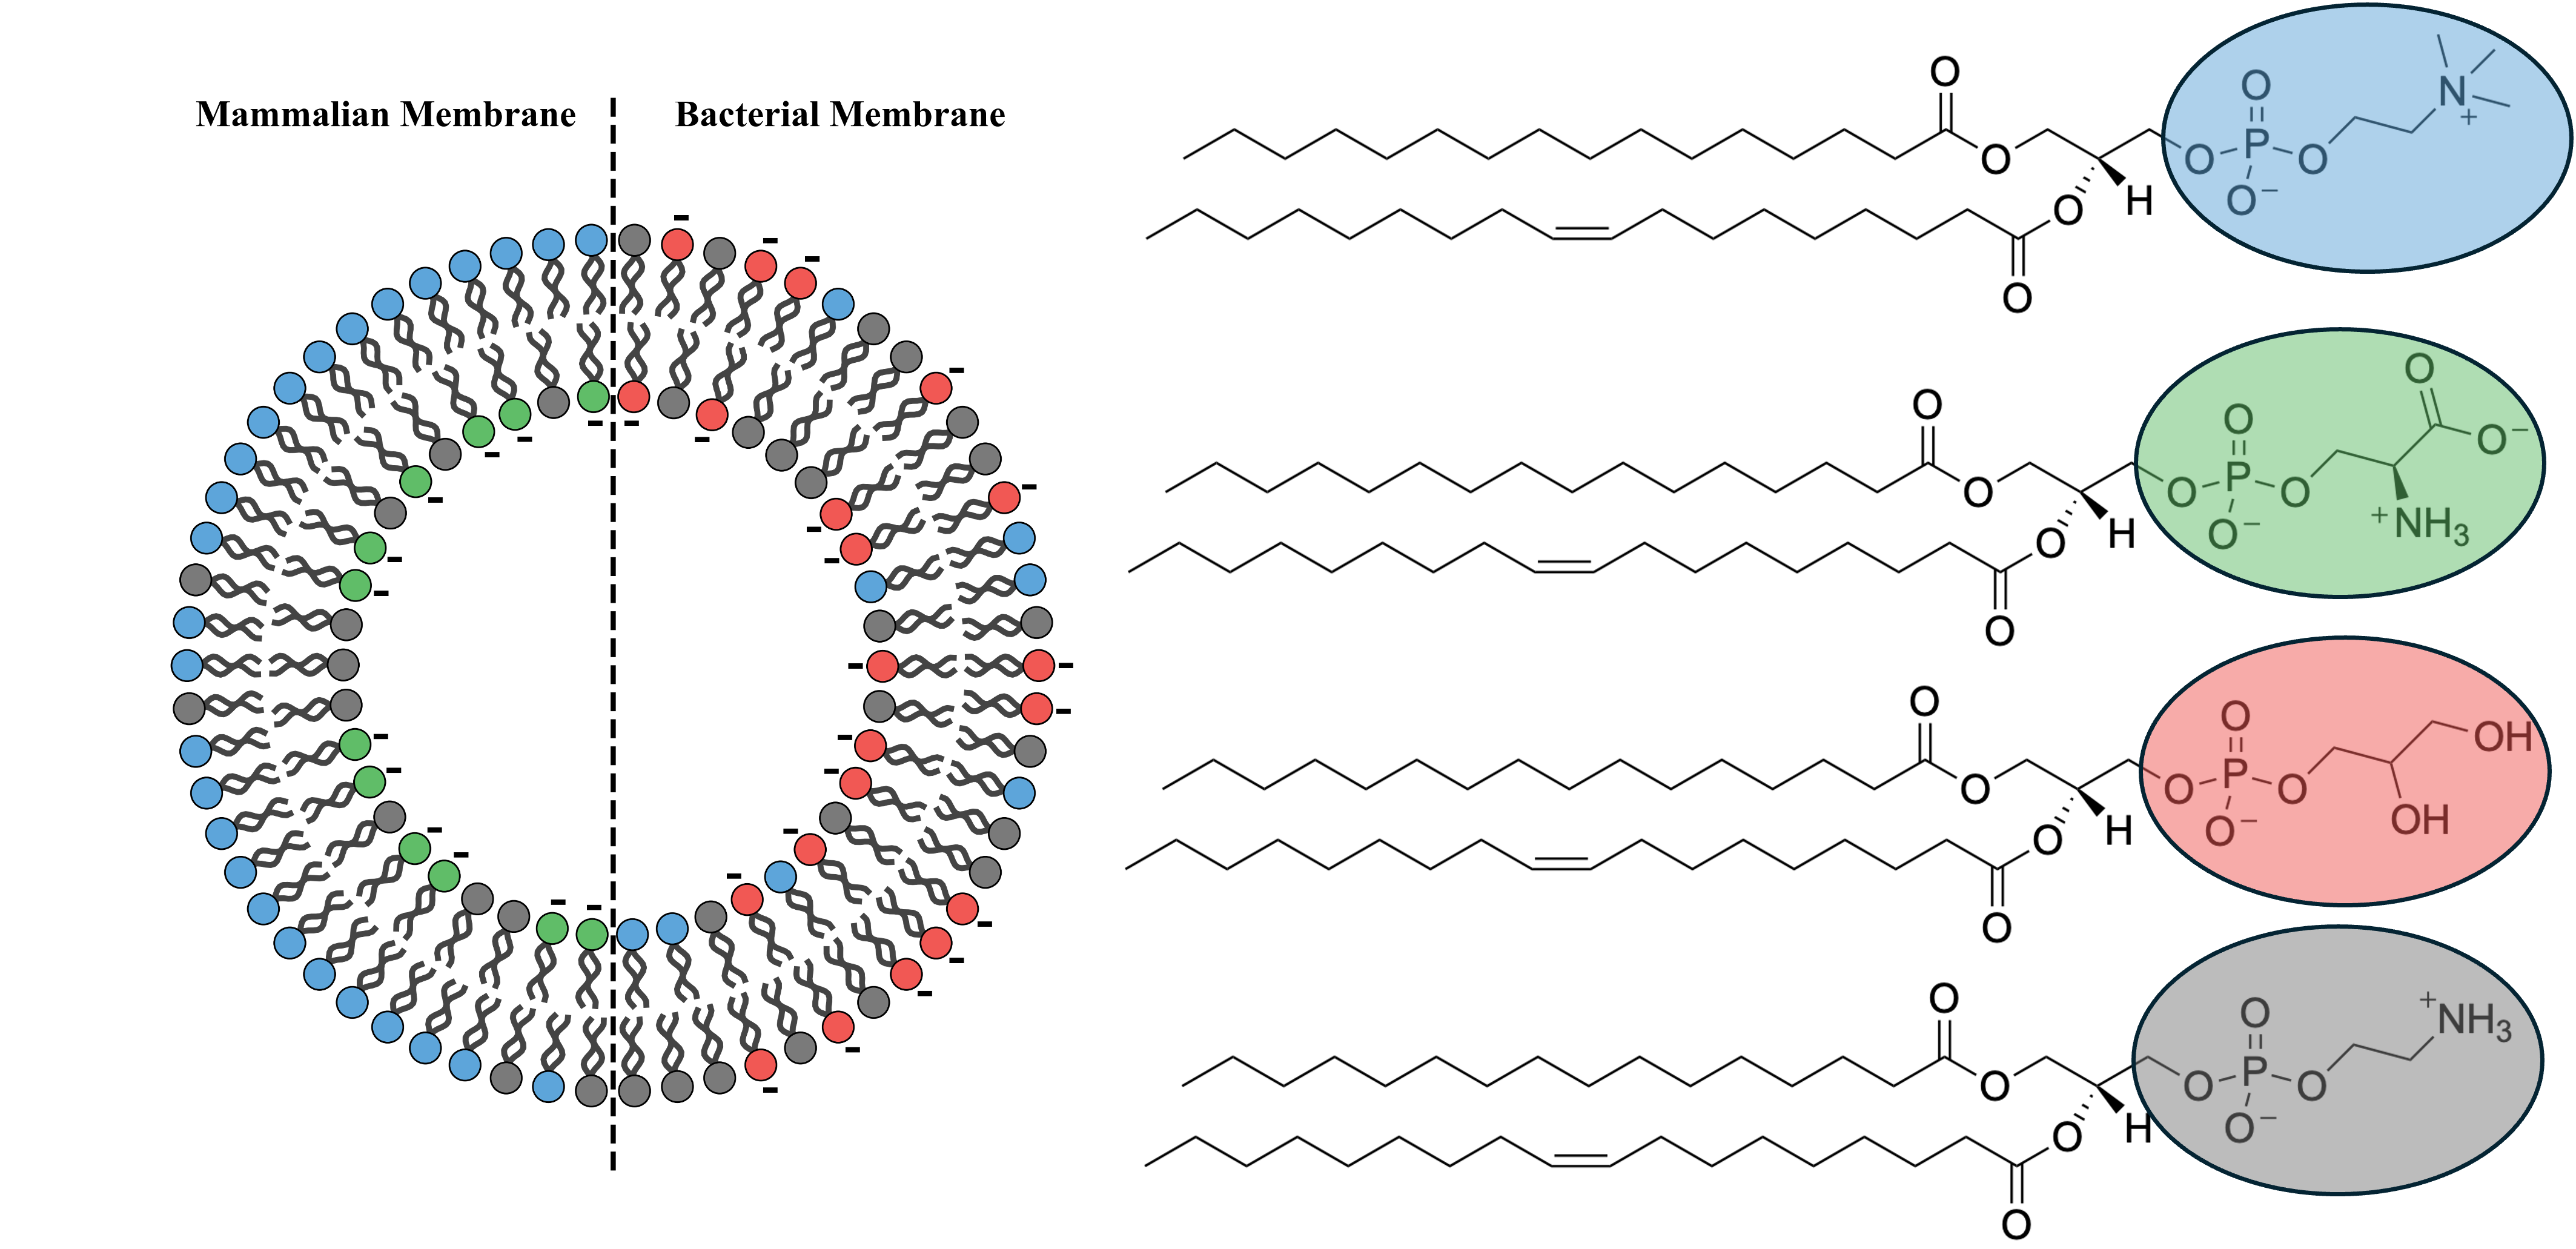
\includegraphics[width=0.95\linewidth]{General_Sections/Figures/Membrane_Lipids.png}
    \caption{The scheme in the left shows the comparison of the lipid composition of mammalian cells and bacteria membranes. In a healthy mammal, the membrane presents lipid asymmetric: the outer leaflet is primarily composed of neutral phosphatidylcholines (blue), while the inner leaflet is enriched with phosphatidylethanolamines (gray) and anionic phosphatidylserines (green), which provide a net negative charge. On the other hand, bacteria contain mainly---both in the interior and exterior leaflet---phosphatidylethanolamines and anionic phosphatidylglycerols (red) making them negatively charged. The structures in the right represent the most common lipids in eukaryotic and bacteria cells. From top to bottom DMPC, DMPS, DMPG, and DMPE. The left figure was created using Matplotlib, while the molecular structures were sketched with ChemDraw.}
    \label{fig:Lipids}
\end{figure}
\FloatBarrier

In the search for new antimicrobial strategies, nature provides an important source of inspiration. As part of their innate immune systems, many animals and plants produce antimicrobial peptides (AMPs) across a variety of tissues and cell types \cita{Zasloff2002}. These peptides have attracted particular interest due to their ability to exploit fundamental physicochemical differences between bacterial and eukaryotic membranes, and are often hypothesized to interact preferentially with membrane compositions enriched in negatively charged lipids\cita{Midura-Nowaczek2014}.

\section{Antimicrobial Peptides}
Antimicrobial Peptides are a class of small peptides that are widely found in nature. They exhibit structural and functional diversity and are active against Gram-positive and Gram-negative bacteria, fungi, parasites, and viruses \cita{Hancock2006}\textsuperscript{,}\cita{Kumar2018}. AMPs typically consist of 10 to 60 amino acids, and almost all AMPs are cationic, although several anionic AMPs have been reported, with up to 187 entries listed in the antimicrobial peptide database APD3 as of December 2024 \cita{Wang2016}. The diversity of AMPs makes their classification difficult, which can be based on: source, activity, structural characteristics, and amino acid-rich species (Figure \ref{fig:AMPClass})\cita{Huan2020}.
% \FloatBarrier
\begin{figure}[h]
    \centering
    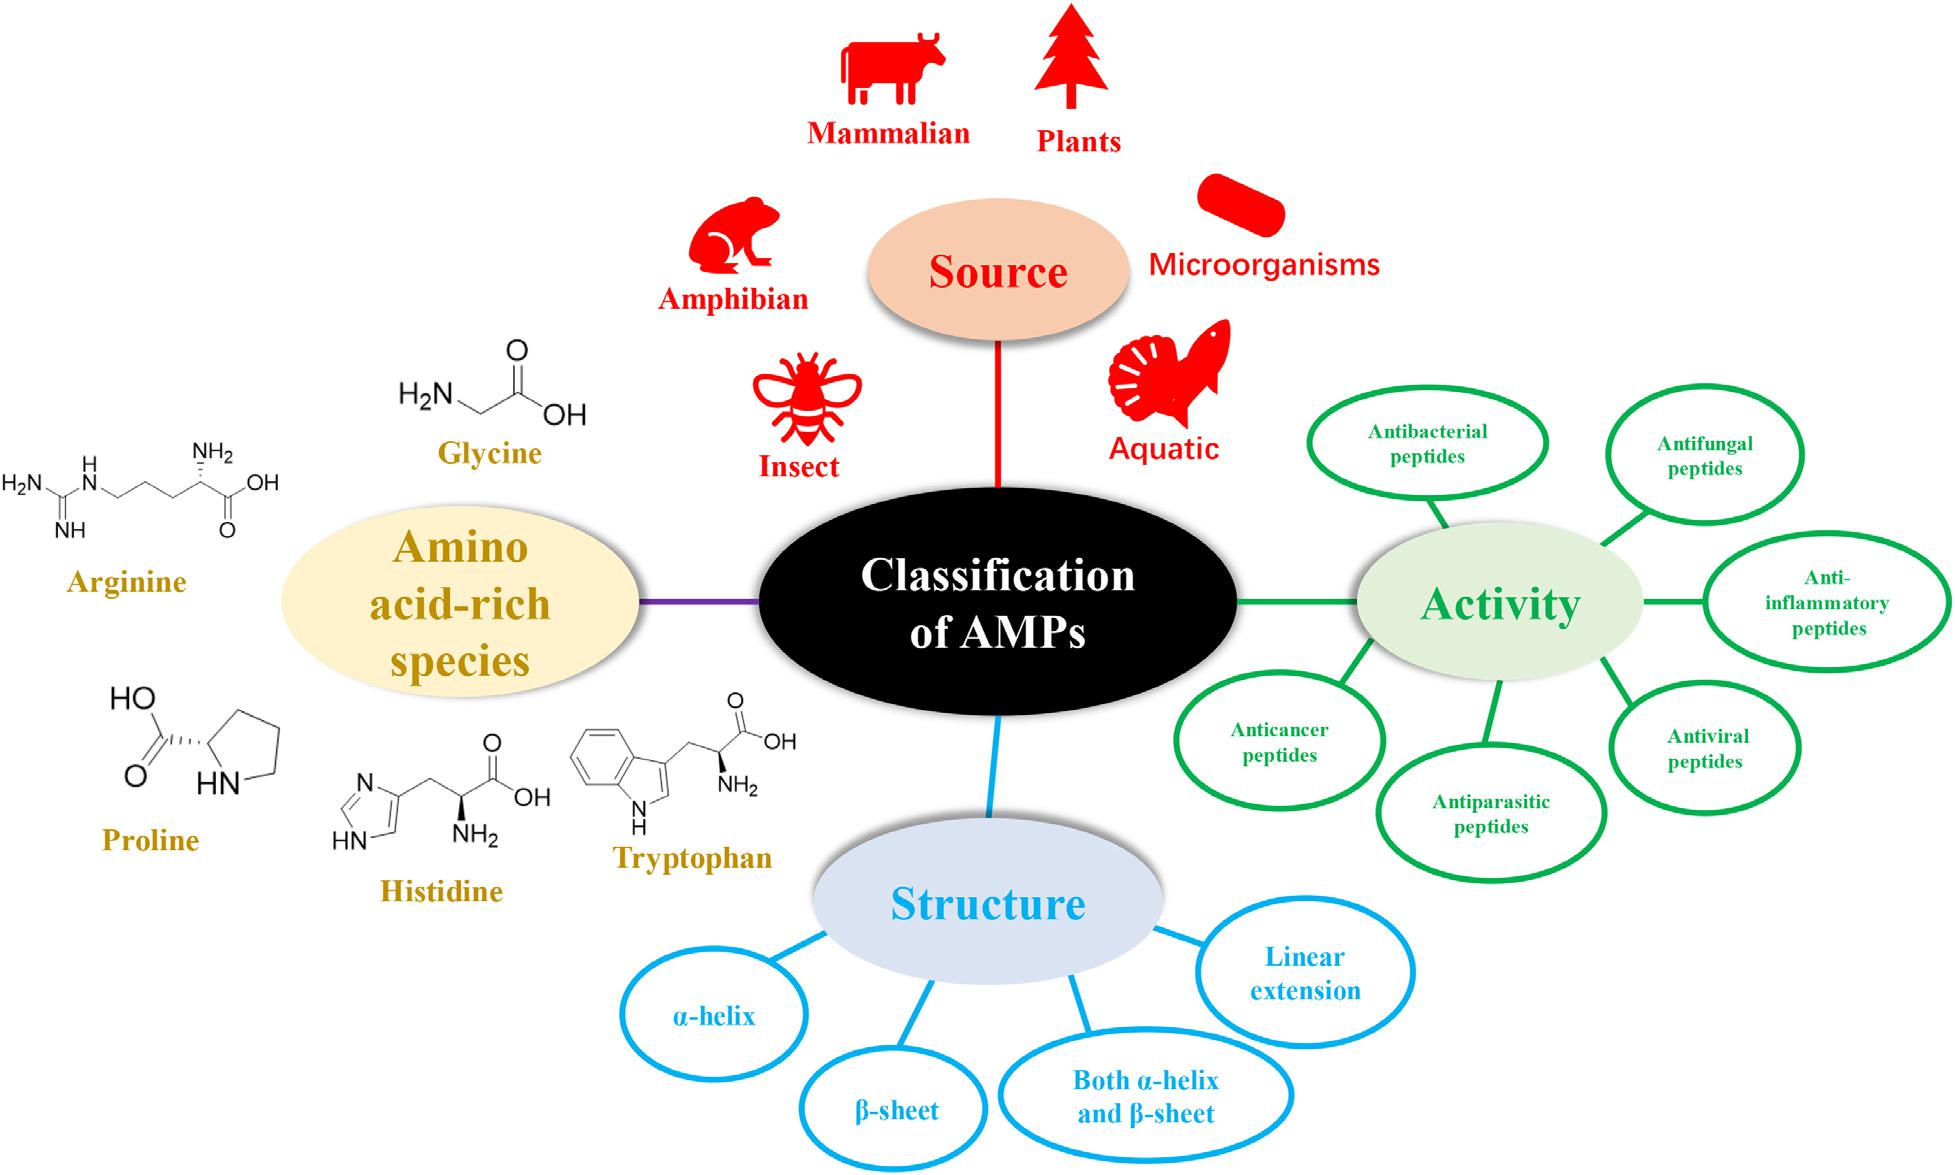
\includegraphics[width=0.8\linewidth]{General_Sections/Figures/AMP_Classification.jpg}
    \caption{Classification of Antimicrobial Peptides. Image taken from the work of Huan, Y. \textit{et al} under a Creative Commons License.}
    \label{fig:AMPClass}
\end{figure}
% \FloatBarrier

Their biological activity is commonly linked to their cationic nature, which allows electrostatic interactions with the negatively charged membranes of invading pathogens rather than with the neutrally charged membranes of eukaryotic cells \cita{Zhang2021}. Additionally, hydrophobicity---defined as the percentage of hydrophobic residues---is another key feature, as it influences the ability of AMPs to partition into membrane lipid bilayers \cita{Yeaman2003}. AMPs usually present a hydrophobicity of around 50\%, which, together with their cationicity, typically leads to amphipathic structures. In many cases, AMPs are largely unstructured in aqueous solution but undergo a conformational transition to $\alpha$-helical structures upon interaction with lipid membranes, a process that enhances their amphipathic character and membrane-disruptive potential \cita{Li2021}. While some AMPs display their antimicrobial activity by means of non-lytic mechanisms \cita{Scocchi2016}, the most common modes of action involve membranolytic effects driven by their amphiphatic nature (Figure \ref{fig:AMPMOA}). In a first stage, electrostatic interactions with negatively charged components of the membranes promote the accumulation of AMPs. Next, the membrane’s non-polar core interacts with the peptides’ hydrophobic residues, facilitating their insertion, disturbing membrane structure, and ultimately leading to cell death\cita{Mookherjee2020}\textsuperscript{,}\cita{BuiThiPhuong2024}.

\begin{figure}[h]
    \centering
    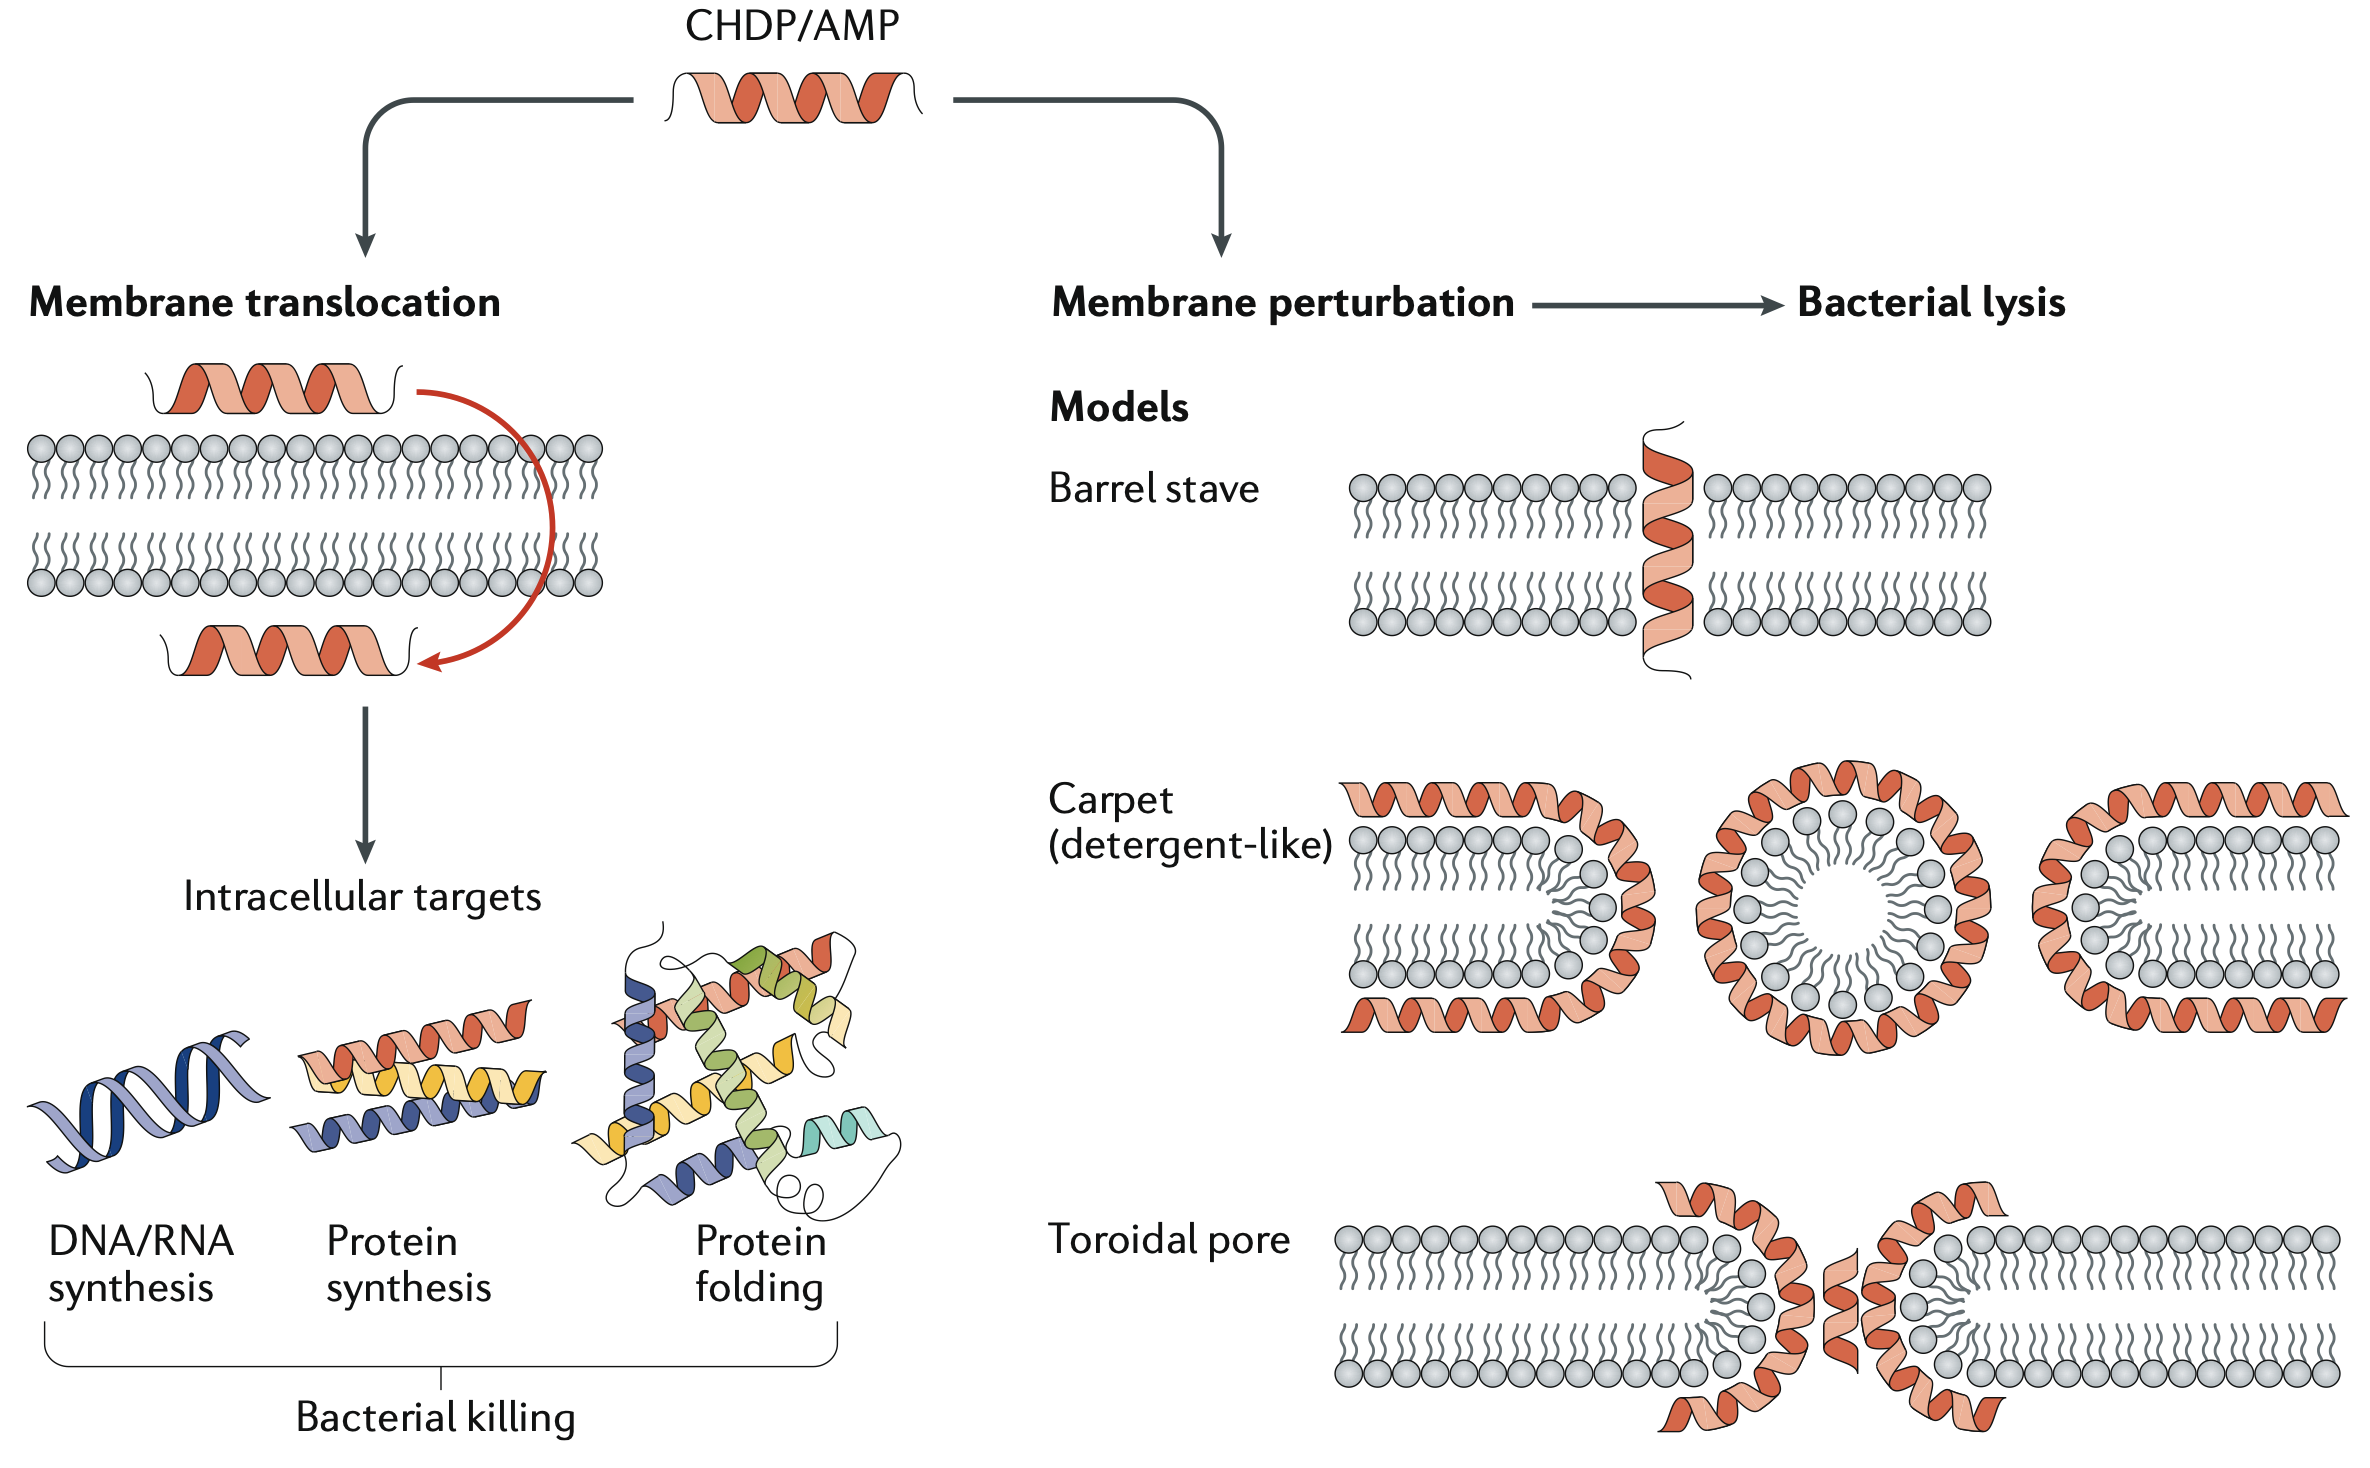
\includegraphics[width=0.69\linewidth]{General_Sections/Figures/AMPMOA.png}
    \caption{Indirect (non-lytic) and direct (membrane-related) mechanisms of bacterial killing proposed for AMPs. Image taken from the work of Mookherjee, N. \textit{et al}, copyright by Springer Nature.}
    \label{fig:AMPMOA}
\end{figure}
\FloatBarrier

As of its latest update in December 2024, the Data Repository of Antimicrobial Peptides (DRAMP)\cita{Ma2025} lists 35918 entries under the query "antimicrobial". Nevertheless, only a few AMPs have reached clinical trials, and just 80 peptide-based drugs have been approved worldwide\cita{Rossino2023}. A major limitation of AMPs is their metabolic instability, as they are rapidly degraded by proteolytic enzymes\cita{Dijksteel2021}. They also tend to exhibit toxicity toward host cells, which limits their therapeutic application\cita{Lyu2023}. In addition, they tend to have short half-lives and are quickly cleared from the bloodstream, which results in poor bioavailability. To overcome these limitations, various strategies have been investigated, such us incorporating non-natural amino acids and peptide cyclization to improve stability and minimize degradation\cita{Carmona2013}\textsuperscript{,}\cita{Lucana2021}.

In this context, there are already cyclic versions of AMPs that exhibit good activity \cita{Mika2011}\textsuperscript{,}\cita{Abraham2014}, highlighting CPs as a promising strategy to enhance natural AMPs or to design new sequences to mimic their function.
 
\section{Self-Assembled Cyclic Peptide Nanotubes}
Researchers, in their continuous effort to push the boundaries of science, have envisioned CPs not only as a means to improve AMPs, but also as promising building blocks for the formation of nanotubular structures driven by noncovalent interactions\cita{Chapman2012}. 

The first self-assembled cyclic peptide nanotubes (SCPNs) were synthesized by Ghadiri in 1993, almost 20 years after they were first proposed by De Santis in 1974\cita{Ghadiri1993}\textsuperscript{,}\cita{DeSantis1974}. These CPs were formed by an even number of alternating \textit{D-} and \textit{L-}$\alpha$-amino acid residues. The alternating chirality leads to a flat, ring-shaped molecule, leaving the oxygens of the carbonyl groups (C=O) and the hydrogens of the amine groups (NH) oriented perpendicular to the plane of the CP. This unique geometry allows CPs to self-assemble by forming hydrogen bonds (H-bonds) with adjacent CPs, mimicking a $\beta$-sheet arrangement (Figure \ref{fig:SCPN}A).

\begin{figure}[htbp]
  \centering

  % Top image (A)
  \begin{subfigure}{0.6\textwidth}
    \centering
    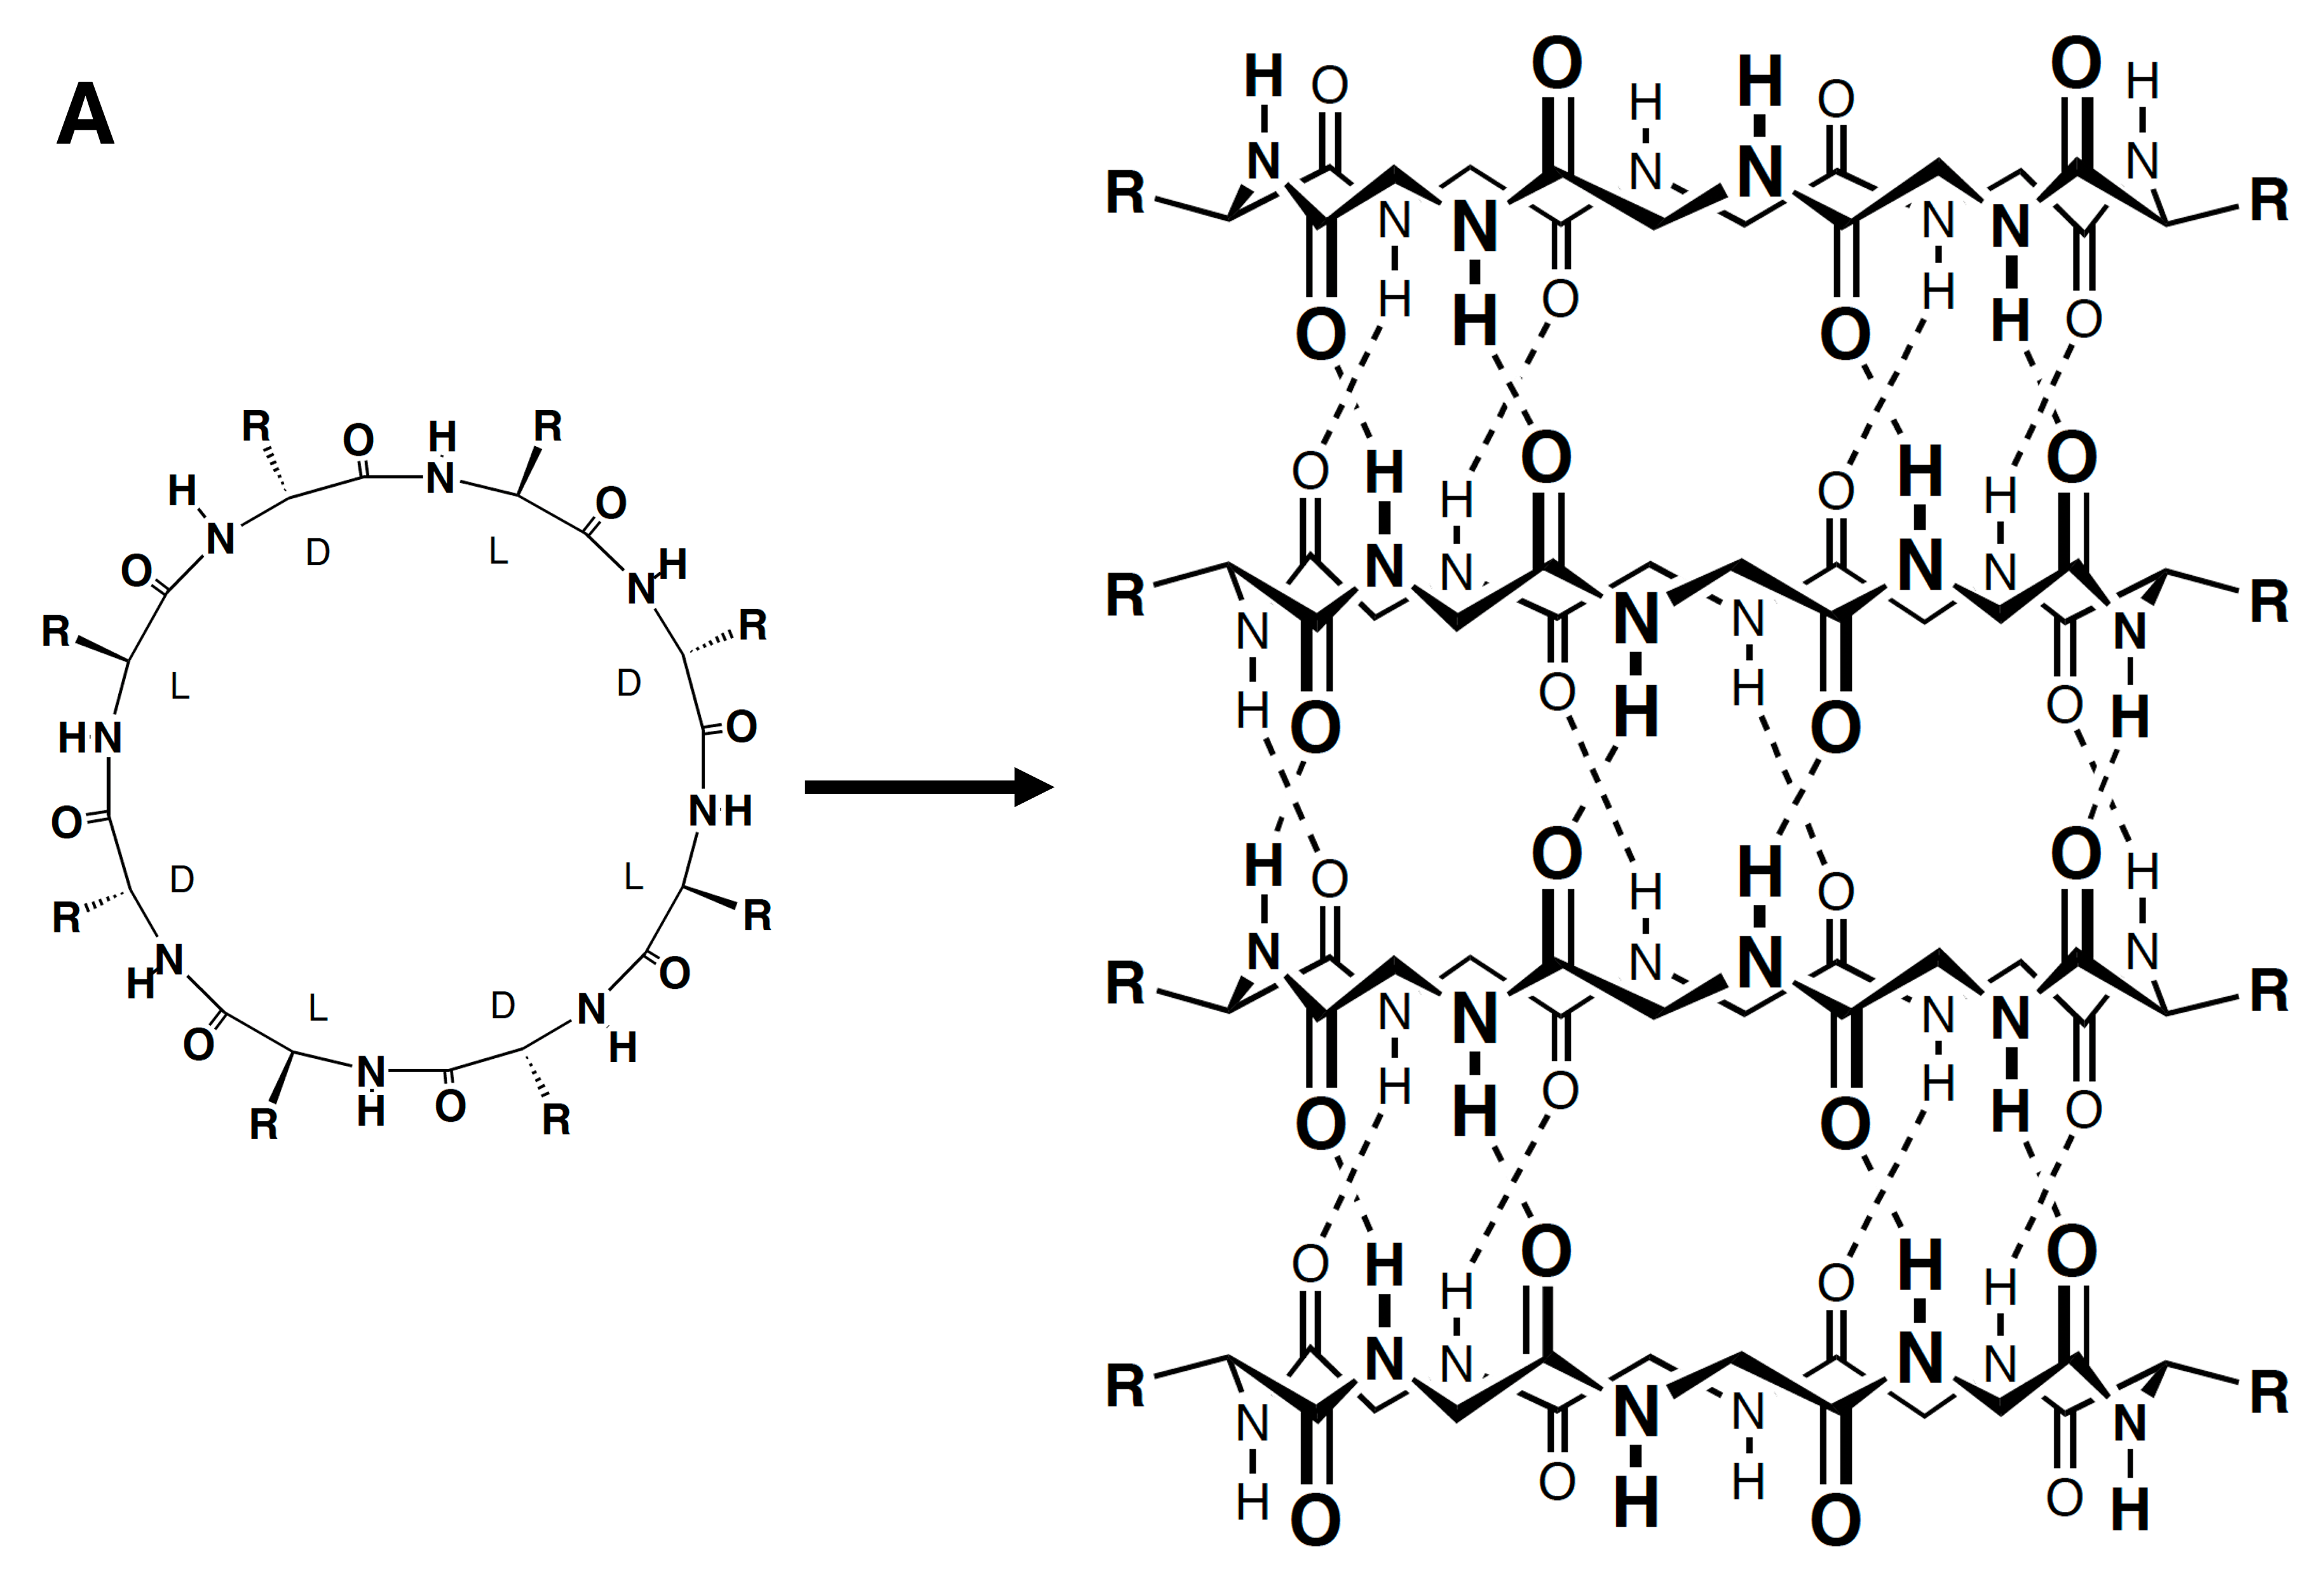
\includegraphics[width=\linewidth]{General_Sections/Figures/SchematicSCPN.png}
  \end{subfigure}

  % \vspace{1em} % vertical space between the two images

  % Bottom image (B)
  \begin{subfigure}{0.6\textwidth}
    \centering
    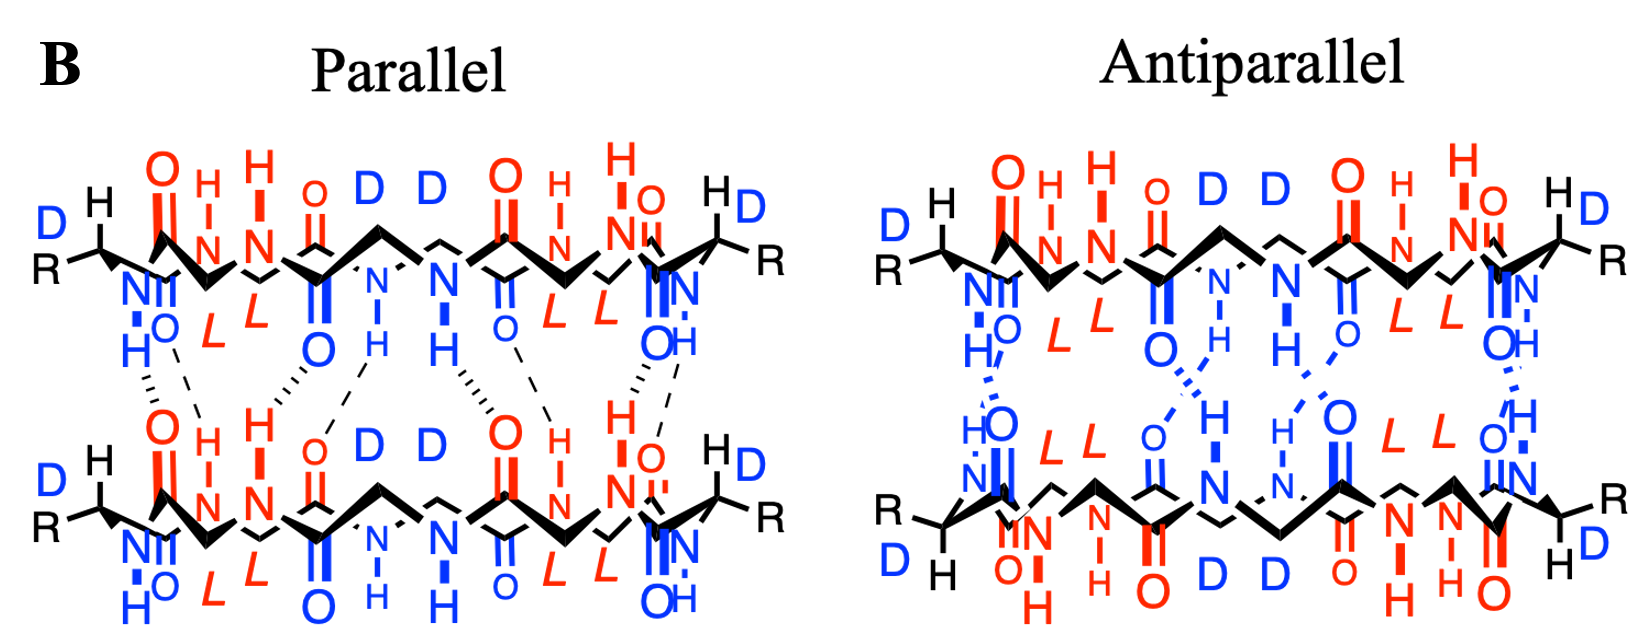
\includegraphics[width=\linewidth]{General_Sections/Figures/PvsA.png}
  \end{subfigure}

  \caption{\textbf{A} Schematic representation of a \textit{D,L-}$\alpha$-C and the corresponding assembly in a SCPN. \textbf{B} Representation of the parallel and antiparallel $\beta$-sheets formed by CPs.}
  \label{fig:SCPN}
\end{figure}

Furthermore, in this planar conformation, all the C=O and NH groups of residues with the same chirality point in the same direction, giving rise to two distinct faces: a \textit{D-}face and a \textit{L-}face. This allows two CPs to assemble by forming either parallel or antiparallel $\beta$-sheet-like structures (Figure \ref{fig:SCPN}B).

The resulting SCPNs have an internal cavity and an external surface, whose properties can be tailored during CP synthesis. The internal diameter can be adjusted by increasing the number of amino acids in the sequence. Moreover, hydrophobicity can be tuned by replacing some of the $\alpha$-residues with $\beta$-amino acids\cita{Claro2018} or $\gamma$-/$\delta$-cycloalkyl-like amino acids\cita{Amorn2003}\textsuperscript{,}\cita{Lamas2018}. In contrast, the nature of the external surface is determined by the choice of amino acids, and this has been observed to dictate the behaviour of the SCPNs in the presence of lipid bilayers, thereby shaping their applications.

In 1994, Ghadiri's group showed that CPs with hydrophobic side-chains, such as Leu or Trp, could self-assemble within lipid bilayers (Figure \ref{fig:Assembly}), forming transmembrane channels capable of ion transport \cita{Ghadiri1994}\textsuperscript{,}\cita{Kim1998}. Subsequent studies revealed that the use of amphipathic CPs with well differentiated hydrophobic and hydrophilic regions, could align parallel to the surface of the membrane (Figure \ref{fig:Assembly}), showing good antimicrobial activity \cita{Fernandez-Lopez2001}. These findings highlight the potential to tune SCPN-membrane interactions through CP sequence engineering.

\begin{figure}[h]
    \centering
    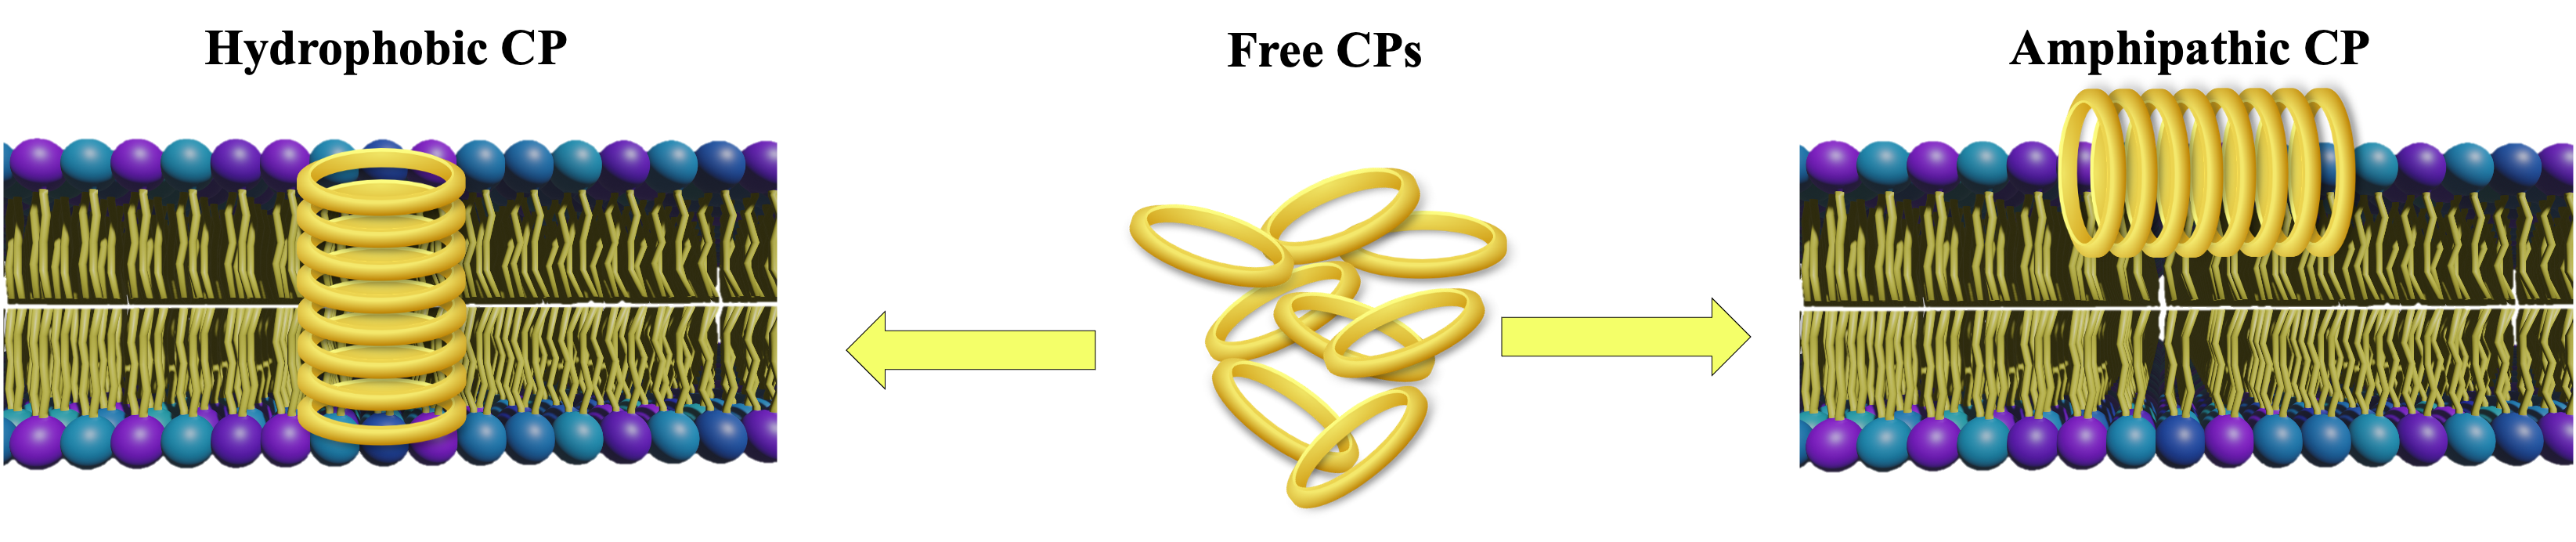
\includegraphics[width=0.9\linewidth]{General_Sections/Figures/DirectedAssembly.png}
    \caption{Representation of the disposition relative to the membrane adopted by hydrophobic SCPNs (left) and amphipathic SCPNs (right).}
    \label{fig:Assembly}
\end{figure}
\FloatBarrier

To effectively design SCPNs to exhibit specific properties or biological functions, it is important to decipher their mechanisms of action. This demands atomic-level resolution, which remains challenging for most experimental techniques. Furthermore, SCPNs---like other supramolecular systems---are highly dynamic. Thus, to fully understand the relationship between sequence, structure, and function, it is necessary to observe how these molecules interact with themselves and their environment in real time. Without the capability to understand the dynamic behavior and structural changes that define their activity, their design must rely on empirical approaches, as well as on serendipity. In this regard, computational techniques and, in particular, Molecular Dynamics (MD), have already proven to be useful tools to advance our understanding of SCPNs \cita{Moral2023}\textsuperscript{,}\cita{Insua2023}.

\section{Computational Methods in Chemistry}

As the performance of computational methods is tightly linked to the available computational power, advances in supercomputing and simulation techniques are pushing the boundaries of molecular simulations of biological systems. In parallel, the breakthrough of Artificial Intelligence (AI) is revolutionizing science, by enabling the analysis of huge databases to make accurate predictions. In the field of molecular biophysics and chemistry, MD simulations and ML approaches are increasingly recognized as complementary tools. While ML models have already demonstrated the ability to predict properties such as CP membrane permeability directly from experimental data \cita{Cao2024}\textsuperscript{,}\cita{Yu2024}, MD simulations provide a unique advantage by generating physically consistent, time-resolved trajectories that describe molecular structure, dynamics, and interactions under well-defined conditions. This makes MD-derived data particularly suitable for training and validating ML models, especially in systems where experimental characterization is challenging. This synergy between Molecular Dynamics and Artificial Intelligence is the main foundation of this doctoral thesis. By combining physics-based modeling with data-driven approaches, this work aims to bridge molecular-level mechanisms and predictive capabilities, contributing to emerging paradigms in computational chemistry.

\subsection{Molecular Dynamics}

MD is a simulation technique used to study the evolution over time of molecular systems by explicitly modeling the motion of atoms or interaction sites through the numerical integration of Newton’s equations of motion. At each time step, the forces acting on the particles are computed using force fields, a set of equations and parameters that describe different inter and intramolecular interactions \cita{Ciccotti2022}.

The first MD simulation dates back to 1957, when Wainwright and Alder simulated systems of hard spheres using a discontinuous potential \cita{Alder1957}. The next step was taken by Rahman in 1964, who simulated liquid argon using a Lennard-Jones pairwise additive potential to account for the interactions between argon atoms. During an era in which computers were scarce and limited in speed and memory, advances in algorithms were essential. In 1967, for example, Verlet proposed a stable numerical integration scheme for Newton's equations, an approach that is still widely used today \cita{Verlet1967}. Later on, in 1971, Rahman and Stillinger published for the first time an MD study on a model of liquid water \cita{Rahman1971}, demonstrating that its structure is formed by a dynamic network of hydrogen bonds. Although today this may seem like routine work, at the time it led the scientific community to believe that if it was possible to simulate water, the medium of the chemistry of life, why not simulate biomolecules themselves? The breakthrough came in 1977, when a group led by Karplus published the first MD simulation of a simple protein \cita{McCammon1977}.

During the early 1980s significant progress was made in developing algorithms to sample conditions relevant to experiments. Standard MD simulations operate in the microcanonical (constant energy) ensemble, since Newton's equations of motion conserve the total energy. Andersen was the first to propose a method for achieving constant-pressure MD simulations by extending the dynamical variables of the system to include the volume \cita{Andersen1980}. He was later followed by Parrinello and Rahman, who extended the scheme to include shape fluctuations as well \cita{Parrinello1980}\textsuperscript{,}\cita{Parrinello1981}. Building on Andersen's work, Nosé introduced a new dynamical variable, coupling the kinetic energy of the atoms to the external temperature, allowing MD to sample the canonical ensemble \cita{Nose1984}. Hoover later refined this approach leading to what is known as Nosé-Hoover thermostat \cita{Hoover1985}, widely used in MD simulations today.

Since then, both the size of the simulated systems and the simulation times have grown exponentially, making it common to find studies in the literature on proteins, DNA/RNA complexes or self-assembly processes such as micelle formation \cita{Karplus2002}\textsuperscript{,}\cita{Sponer2018}\textsuperscript{,}\cita{Morrow2013}. More broadly, the impact of molecular simulation approaches on chemical research was formally recognized with the award of the 2013 Nobel Prize in Chemistry to Martin Karplus, Arieh Warshel and Michael Levitt for "the development of multiscale models for complex chemical systems".
%%%
Within this broader landscape, MD simulations have also been applied to the study of cyclic peptides (CPs) and self-assembled cyclic peptide nanotubes (SCPNs), providing molecular-level insight into their conformational behavior, self-assembly mechanisms, and interactions with lipid membranes. Atomistic MD studies offer a level of structural and dynamical detail difficult to access experimentally, helping to elucidate how peptide sequence, chirality, and amphipathicity influence supramolecular organization. Despite these capabilities, previous research in our group has focused specifically on embedded nanotubes, investigating their stability and implications for membrane structure \cita{GF2016}\textsuperscript{,}\cita{Calvelo2019}\textsuperscript{,}\cita{Xandre2021}\textsuperscript{,}\cita{Conde2022}. A shared feature of the cited works was the use of pre-assembled nanotubes that were manually inserted into lipid bilayers, a necessity driven by the high computational cost of the application of atomistic MD to CP and SCPN systems. Key processes such as peptide self-assembly, membrane insertion, and supramolecular rearrangement typically occur on microsecond to millisecond timescales and involve large peptide–membrane assemblies, placing them beyond the practical reach of routine atomistic simulations.

To overcome these limitations, coarse-grained (CG) Molecular Dynamics approaches have been increasingly adopted, as they enable the simulation of larger systems over longer timescales. CG models have been successfully applied to study the interactions of various CP sequences with lipid bilayers, starting either from a pre-assembled nanotube in solution or from randomly positioned units that self-assemble \cita{Claro2020}\textsuperscript{,}\cita{Claro2021}. However, while CG models are well suited to capture collective phenomena such as aggregation and membrane remodeling, their reduced resolution often compromises the accurate description of direction-specific interactions, including hydrogen-bond networks, backbone geometry, and chirality-dependent stacking. These features are particularly critical for CPs and SCPNs, whose self-assembly is governed by highly directional hydrogen bonding and precise geometric constraints. As a result, existing CG force fields may fail to faithfully reproduce key aspects of cyclic peptide self-assembly and membrane interactions, despite their favorable computational efficiency.

This gap between atomistic accuracy and CG scalability highlights the need for computational strategies that preserve essential structural features of cyclic peptides while enabling systematic, large-scale simulations and data-driven analysis.

Looking forward, MD continue to benefit from advances in high-performance computing, including the deployment of exascale architectures, which enable increasingly large and long simulations of complex molecular systems. In parallel, the breakthrough of AI, and in particular Machine Learning (ML), is profoundly revolutionizing the field. Beyond their application as classification or prediction tools, ML-based approaches are increasingly integrated into the core of theoretical chemistry through the development of ML potentials, which offer a promising route to accelerate MD while preserving atomic accuracy.


\subsection{Machine Learning}\label{ML_intro}
%%%%%% CONTINUE
Although commonly confused in everyday conversations, AI and ML refer to distinct but interconnected concepts. AI describes the field of study dedicated to enabling computers and machines to simulate human intelligence and capabilities, performing tasks such as reasoning or decision-making. ML constitutes a major subfield of AI, concerned with developing models by training algorithms to make predictions based on data rather than explicitly programming them to provide an outcome.

The term Machine Learning was coined by Arthur Samuel in the late 1950s, when his computer program for playing checkers was one of the first successful self-learning programs \cita{Samuel2000}. In parallel, Frank Rossenblatt, inspired by Donald Hebb's model of brain cell interaction \cita{Hebb2005}, developed a simple neuron-inspired classifier called the perceptron \cita{Rosenblatt1958}. The software was installed in a custom-built machine called the Mark I Perceptron, which had been constructed for image recognition. Despite early promise, its limitations in recognizing some visual patterns led to disappointment and temporarily stalled progress in neural network research.

A resurgence came in the 1980s as the development of new training algorithms and increased computational power unlocked multi-layer neural networks. In 1986, Rumelhart, Hinton, and Williams popularized the back-propagation algorithm that enabled networks to adjust internal weights in hidden layers, learning feature representations beyond the perceptron's reach \cita{Rumelhart1986}. In the 1990s, Hochreiter and Schmidhuberthe developed the Long Short-Term Memory (LSTM) networks that addressed the long-standing vanishing gradient problem that was burden recurrent networks. LSTMs soon achieved state-of-the-art performance on sequential data tasks, breaking records in domains like language modeling and machine translation by the mid-2010s \cita{Hochreiter1997}. By 2017, the confluence of large datasets and Graphics Processing Unit (GPU) computing led to the development of AlexNet, a deep convolutional neural network that scored a landmark victory in the ImageNet recognition challenge \cita{Krizhevsky2017}.

As ML matured, it increasingly intersected with other areas of knowledge like chemistry. For instance, in 2007 Behler and Parrinello showed that a neural network could replicate density functional theory (DFT) potential energy surfaces, providing energies and forces orders of magnitude faster than DFT calculations \cita{Behler2007}. Since then, ML potentials have gained popularity, as they are believe to extend accessible time-scales without sacrificing accuracy. Nevertheless, the most striking example of ML's impact on chemistry has arguably been in protein structure prediction. Predicting protein's 3D structure just based on the amino acid sequence remained unsolved for five decades. In 2020, DeepMind launched AlphaFold2, a neural network capable of predicting protein structures with unprecedented accuracy \cita{Jumper2021}. In recognition, the 2024 Nobel Prize in Chemistry was awarded to Demis Hassabis and John Jumper, creators of AlphaFold, as well as David Baker for his pioneering contributions to computational protein design. This was the first time an AI-driven scientific achievement earned a Nobel Prize, reinforcing that ML is no longer just a computational aid, but an essential tool for advancing chemical research.

In the context of medicinal chemistry and peptide research, ML approaches have been widely employed to predict biological activity, toxicity, and membrane permeability directly from experimental data \cita{Manavalan2018}\textsuperscript{,}\cita{Wang2024}\textsuperscript{,}\cita{Li2024}. Several models have been reported to infer cyclic peptide membrane permeability or antimicrobial activity from sequence-based representations or molecular descriptors, demonstrating the potential of ML to accelerate screening and guide peptide design \cita{CyclePermea}\textsuperscript{,}\cita{Feller2025}\textsuperscript{,}\cita{Tan2024}. However, ML models trained exclusively on experimental datasets often face important limitations. Experimental data is frequently scarce, heterogeneous, and biased toward specific chemical families, which can hinder model generalization and limit interpretability. Moreover, purely sequence-based representations may fail to capture key aspects of molecular behavior that arise from the three-dimensional structure, supramolecular organization, and dynamic interactions with complex environments such as lipid membranes.

In this context, Molecular Dynamics simulations offer a complementary and highly valuable source of training data for ML models \cita{Hui2023}\textsuperscript{,}\cita{Cherednichenko2025}\textsuperscript{,}\cita{Hui2025}. MD provides physically consistent, time-resolved information that encodes not only static structural features but also dynamic, thermodynamic, and interaction-based descriptors. By extracting quantitative features from MD trajectories, it becomes possible to generate large, homogeneous datasets that reflect underlying molecular mechanisms rather than purely empirical correlations.

The integration of ML with MD simulations opens new opportunities for bridging molecular-scale mechanisms and macroscopic observables. ML models trained on simulation-derived descriptors can learn complex relationships between sequence, structure, dynamics, and function, enabling rapid prediction and classification at a fraction of the computational cost of explicit simulations. For cyclic peptides and self-assembled cyclic peptide nanotubes, this combined MD–ML framework is particularly attractive, as it provides a route to explore vast sequence spaces while accounting for the supramolecular and membrane-associated phenomena that govern biological activity.


\section{Dissertation Structure}

This PhD dissertation is structured into seven main sections and one supplementary section. The manuscript first delves into the context behind the work, namely, the challenge of AMR, and then presents the molecules and techniques used to address it. After that, the objectives of this research are presented, followed by a technical explanation of the materials and methods used to carry out research. Subsequently, the scientific results are presented as a compendium of articles, comprising the five most relevant publications related to this thesis divided in three results sections. Finally, the contributions are discussed as a whole in order to draw a general list of conclusions. In particular, the document is structured as follows:
\begin{itemize}
    \item \textbf{Introduction}: The present section. It introduces AMR and proposes CPs as potential candidates to overcome it. Additionally, it also describes the scientific challenges of experimental CP research and provides an overview of the two main techniques used in this work: MD simulations and ML methods. 
    \item \textbf{Hypothesis and Objectives}: This section sets the main hypothesis that drive the research conducted in this thesis. Moreover, it provides a detailed description of the objectives that have to be achieved to test the proposed hypothesis.
    \item \textbf{Materials and Methods}: This section describes in detail the computational tools used in this research. It first focuses on MD, providing technical insights into the physical foundation and the force field, a pivotal aspect of the thesis. Then, it delves into Machine Learning, describing the main unsupervised and supervised methods featured in the published work.
    \item \textbf{Results: Published Articles}: This section includes the articles published during the thesis and, when applicable, the corresponding supporting information right after the article. Moreover, this section presents the platform CYCLOPEp, which contains registered code. The corresponding registration form is attached at the end of the article presenting \hyperlink{registro}{CYCLOPEp Builder}, the first tool of CYCLOPEp. The articles are in the original format they were published, including then, the discussion of the results obtained in each research work. Two sections form this chapter; Section \ref{chap1} covers the development of the MA(R/S)\-TINI force field and the creation of CYCLOPEp Builder, an online platform for the creation of CPs and SCPNs for MD simulations; Section \ref{chap3} describes a model trained to predict experimental CP membrane permeability, the results, and the different strategies tested to improve the accuracy.
    \item \textbf{Unpublished Results}: This section encompass the work that could not be published before the presentation of the thesis. Section \ref{chap2} includes the manuscript were CYCLOPEpDB, an in house database of CP-MD simulations, was presented. This article-like manuscript also provides ML results on the prediction of CP-Membrane interactions derived from the MD results. Although this section was placed after the one containing the published articles, the manuscript that it contains was originally intended to be placed between sections \ref{chap1} and \ref{chap3}, since it uses the tools of the former and advances the application of Machine Learning to Molecular Dynamics data before moving to experimental sources. Therefore, throughout all the thesis, it will be treated as if it was a work in between the aforementioned results sections. The supplementary information of this articles is also provided right after.
    \item \textbf{General Discussion}: This section includes a general overview of the results achieved in this thesis, highlighting the main outcomes of each article and how they integrate in the general purpose of this research.
    \item \textbf{Conclusions}: Presents a summary of the key conclusions drawn from the research carried out in this thesis.
\end{itemize}

\newpage